% Figura cuerpo B2: las tres ecuaciones cierran el círculo: cada bloque aporta una decisión y una incógnita
\documentclass[tikz,border=3pt]{standalone}
\usepackage[T1]{fontenc}
\usepackage[utf8]{inputenc}
\usepackage{amsmath}
\usetikzlibrary{arrows.meta,calc,positioning}
\begin{document}
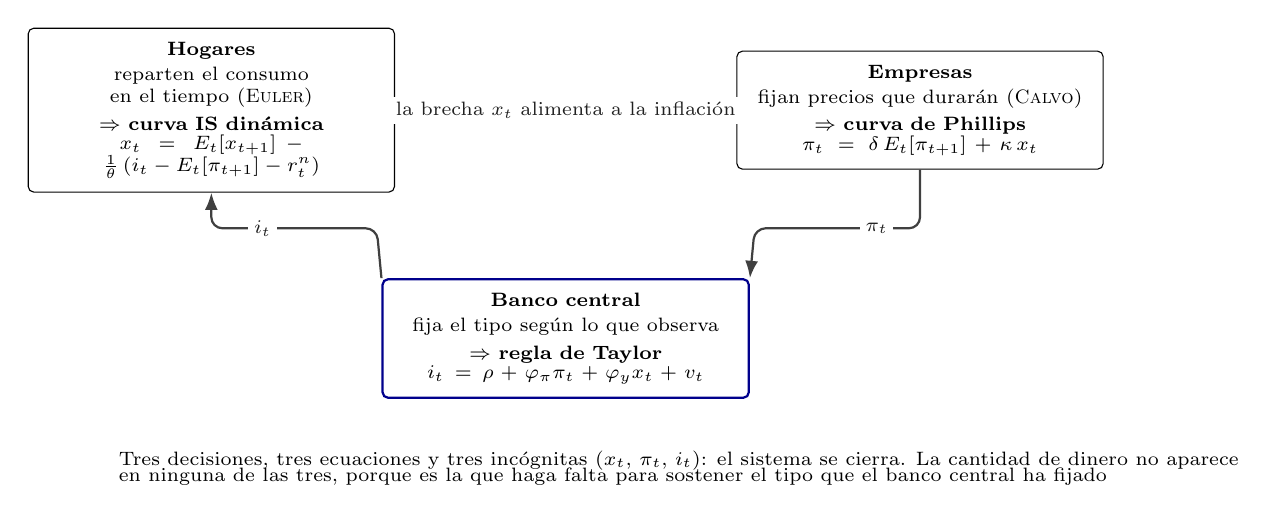
\begin{tikzpicture}[>={Latex[length=2.2mm]}, font=\footnotesize,
  caja/.style={draw, rounded corners=2pt, align=center, inner sep=5pt, text width=4.3cm, font=\scriptsize},
  azul/.style={draw=blue!55!black, thick, rounded corners=2pt, align=center, inner sep=5pt, text width=4.3cm, font=\scriptsize},
  etq/.style={font=\scriptsize, text=gray!25!black, fill=white, inner sep=2pt},
  fl/.style={->, thick, gray!50!black}]
  \node[caja] (h) at (0,3.1) {\textbf{Hogares}\\[1pt]reparten el consumo en el tiempo (\textsc{Euler})\\[2pt]$\Rightarrow$ \textbf{curva IS dinámica}\\[-1pt]$x_{t}=\mathbb{E}_{t}[x_{t+1}]-\tfrac{1}{\theta}\left(i_{t}-\mathbb{E}_{t}[\pi_{t+1}]-r^{n}_{t}\right)$};
  \node[caja] (e) at (9.0,3.1) {\textbf{Empresas}\\[1pt]fijan precios que durarán (\textsc{Calvo})\\[2pt]$\Rightarrow$ \textbf{curva de \textsc{Phillips}}\\[-1pt]$\pi_{t}=\delta\,\mathbb{E}_{t}[\pi_{t+1}]+\kappa\,x_{t}$};
  \node[azul] (b) at (4.5,0.2) {\textbf{Banco central}\\[1pt]fija el tipo según lo que observa\\[2pt]$\Rightarrow$ \textbf{regla de \textsc{Taylor}}\\[-1pt]$i_{t}=\rho+\varphi_{\pi}\pi_{t}+\varphi_{y}x_{t}+v_{t}$};
  \draw[fl] (h.east) -- (e.west) node[etq, midway] {la brecha $x_{t}$ alimenta a la inflación};
  \draw[fl, rounded corners=4pt] (e.south) -- (9.0,1.6) -- (6.9,1.6) -- (b.north east);
  \node[etq] at (8.45,1.6) {$\pi_{t}$};
  \draw[fl, rounded corners=4pt] (b.north west) -- (2.1,1.6) -- (0,1.6) -- (h.south);
  \node[etq] at (0.65,1.6) {$i_{t}$};
  \node[align=left, anchor=north west, font=\scriptsize] at (-1.3,-1.1)
    {Tres decisiones, tres ecuaciones y tres incógnitas ($x_{t}$, $\pi_{t}$, $i_{t}$): el sistema se cierra. La cantidad de dinero no aparece\\[-2pt]en ninguna de las tres, porque es la que haga falta para sostener el tipo que el banco central ha fijado};
\end{tikzpicture}
\end{document}
